\section{MTU Discovery}
\label{sec:MTU Discovery}

\subsection{Einleitung}
todo theo

%TODO: statt Alice und 2 Alice und Bob verwenden!
\subsection{MTU-Bestimmung: Erfolgreich}
Dieses Sequenz-Diagramm stellt den idealen Ablauf bei der MTU-Bestimmung dar. Alice schickt Bob ein Paket mit dem Kommando 'MTU?'. Dieses Paket hat eine typische Grösse gem. Erfahrungswerten. Momentan starten wir mit 500Bytes. %TODO: CITATION NEEDED! GRÖSSE ANPASSEN
Bob erhält das Paket und schickt eine Antwort mit dem Kommando 'OK'. Darauf erhöht Alice
die Grösse des Pakets um einen konfigurierbaren Inkrementationswert und schickt es wieder zurück an
Bob. Dieser Ablauf wird so lange wiederholt bis das Paket nicht mehr bei Bob ankommt.
Weil das Paket nicht ankommt kann Bob keine Antwort senden und Alice läuft in ein Timeout.
Alice nimmt jetzt den letzten erfolgreichen MTU-Wert und schickt Bob erneut ein Paket.
Wenn das Paket erfolgreich ankommt, d.h. Bob ein 'OK' zurückschickt wurde die MTU erfolgreich gefunden. Alice setzt nun einen Meldung ab das die ideal MTU für die Verbindung zwischen Alice und 2 gefunden wurde.

% GFX Trim left bottom right top
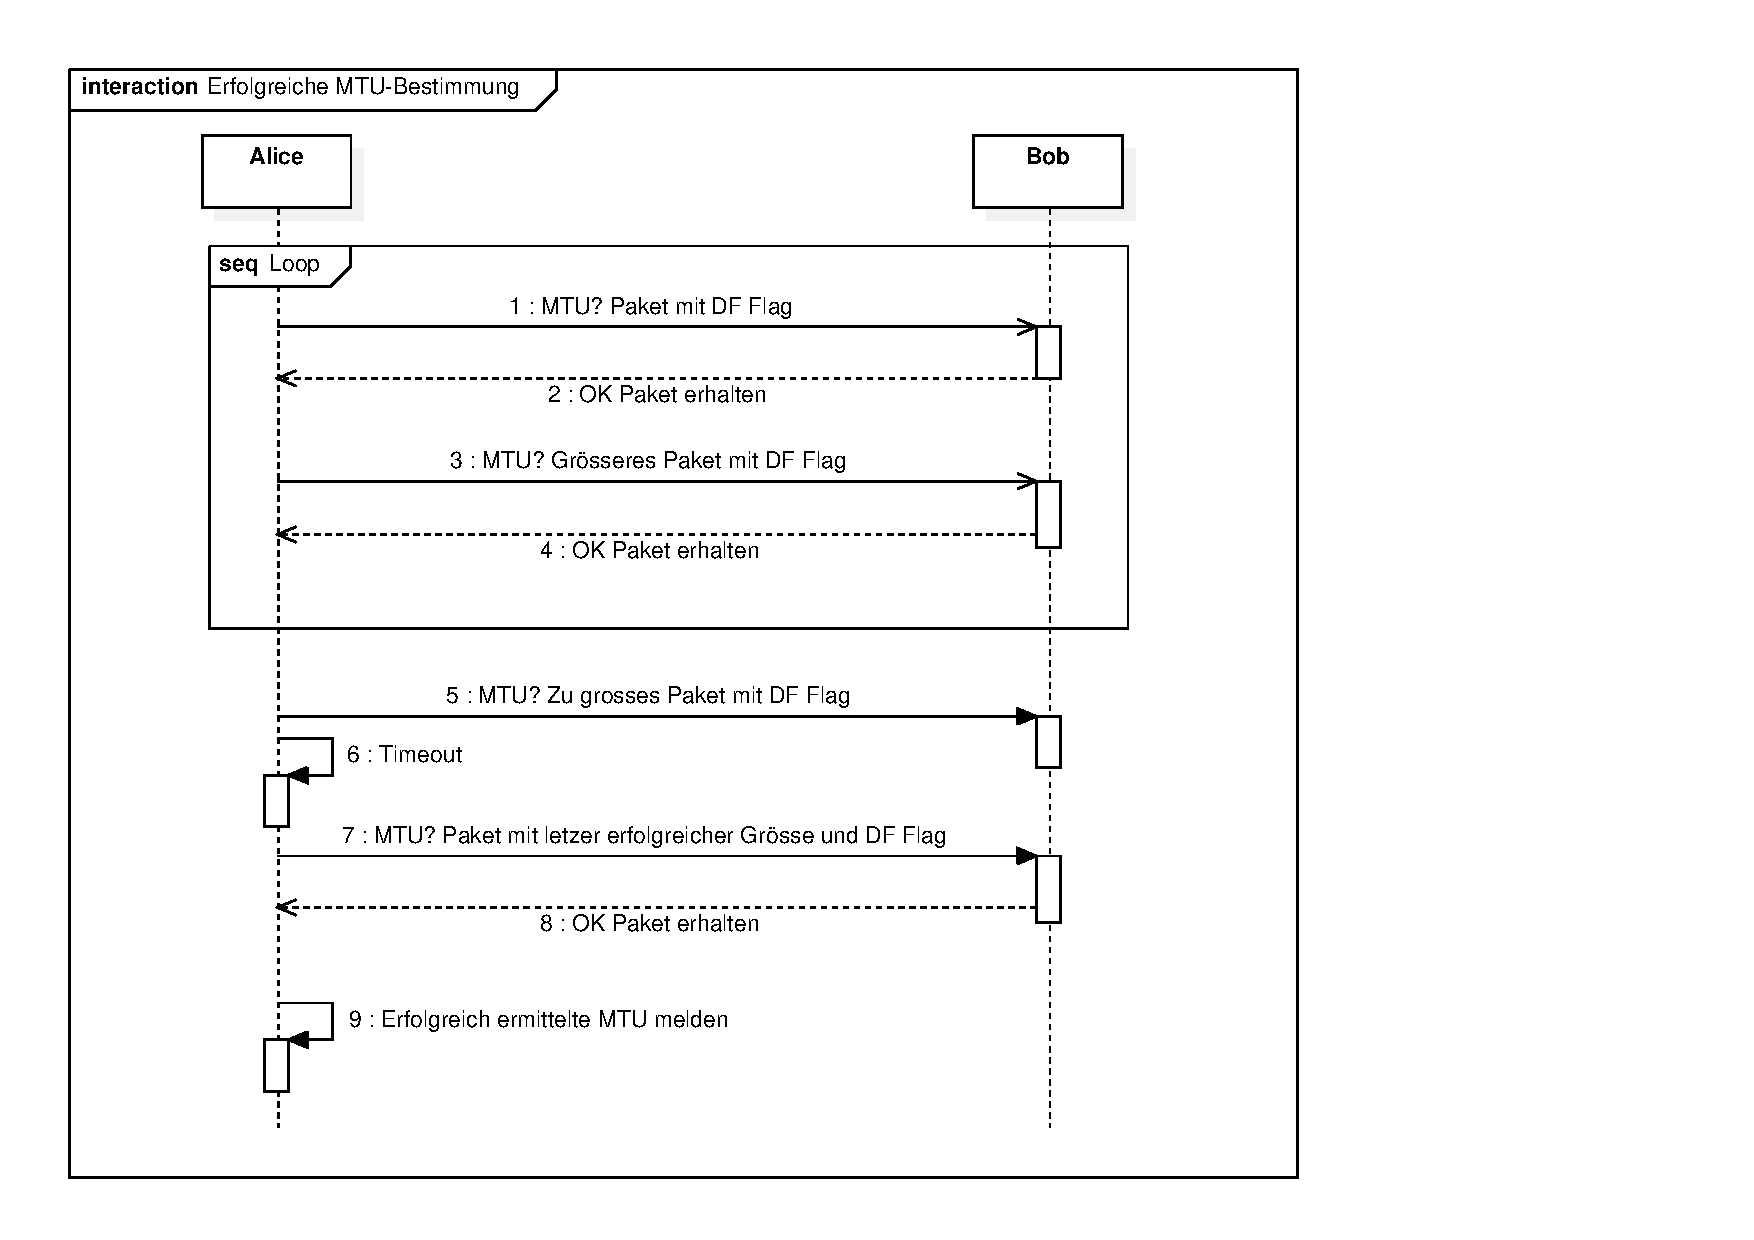
\includegraphics[trim=10 10 200 10,clip,width=\textwidth]{mainpart/implementation/img/MTUBestimmungErfolgreich}

\subsection{MTU-Bestimmung: Fehlerfall}
Dieses Sequenz-Diagramm stellt einen möglichen Fehlerfall bei der Bestimmung der MTU dar. Es zeigt wie das \tool den Fehlerfall behandelt. Alice versucht wie beim erfolgreichen Fall durch das versenden von immer grösseren Paketen die ideale MTU für die Verbindung mit Bob zu finden. Bei Punkt 5 sendet Bob keine Antwort mehr... %TODO: 

% GFX Trim left bottom right top
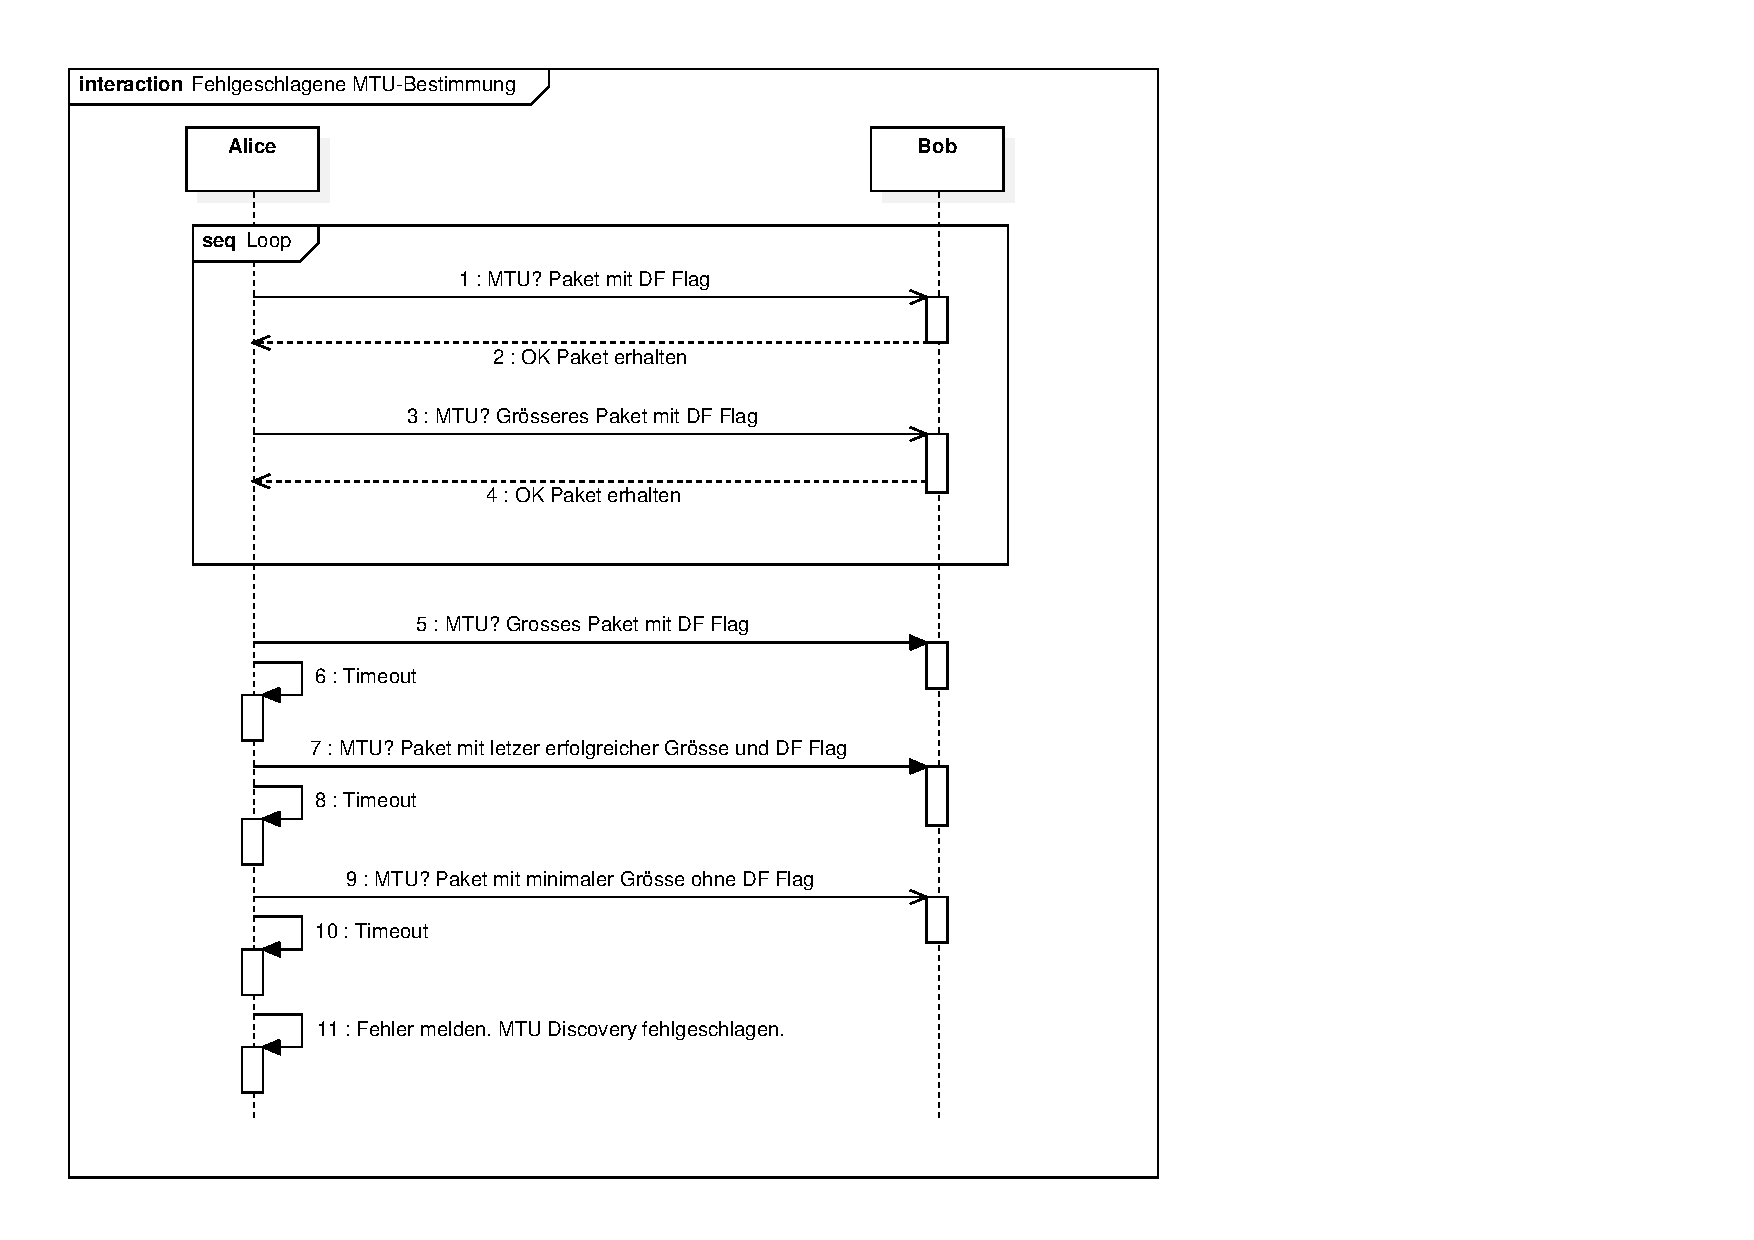
\includegraphics[trim=10 10 265 10,clip,width=\textwidth]{mainpart/implementation/img/MTUBestimmungFehlerfall}